\documentclass[conference]{IEEEtran}
\IEEEoverridecommandlockouts
\usepackage{cite}
\usepackage{amsmath,amssymb,amsfonts}
\usepackage{algorithmic}
\usepackage{graphicx}
\DeclareGraphicsExtensions{.eps,.pdf,.png}
\usepackage{textcomp}
\usepackage{xcolor}
\usepackage{url}
\usepackage{hyperref}
\begin{document}

\title{Research Meeting}

\author{\IEEEauthorblockN{Shun Yamachika}
\IEEEauthorblockA{\textit{Department of Informatics, School of Science and Technology} \\
\textit{Kwansei Gakuin University}\\
Sanda, Hyogo, Japan \\
shun@lsnl.jp}}

\maketitle


\section{LinkSeLFiEの実験設定について}
\label{sec:org8b376ec}
\subsection{P(Point:結論・要点)}
\label{sec:org29df353}
LinkSeLFiEの論文では、均等配分戦略(VanillaNB)は各リンクに過剰な資源
配分を要求するという前提で議論されているが、 各リンクごとの資源配分を
大幅に削減した均等配分戦略(Vanilla 20NB、Vanilla 4NB)がLinkSeLFiEと
同等の性能を劇的に少ない資源で達成しているので、LinkSeLFiEはアルゴリズ
ムの資源効率性における優位性を示せていない。

\subsection{R(Reason:理由)}
\label{sec:org49b5deb}
LinkSeLFiEは、ベースラインである均等配分手法(VanillaNB)に、特に理由
なく過剰な試行回数 T=200(各リンクに2,000バウンス)を設定し、その上で
より少ない資源で同等以上の性能を目指すという形で優位性を示そうとしてい
る。しかしT を大幅に削減した均等配分戦略(Vanilla 20NB、Vanilla 4NB つ
まり各リンクに200バウンス、40バウンス)をLinkSeLFiEと同じ実験設定下で
実験すると以下の結果が得られた。

\begin{itemize}
\item 最適リンクの判別率: Vanilla 4NB、Vanilla 20NBはLinkSeLFiEと同程度の
最適リンク判別率を達成。

\item 量子資源消費: Vanilla 20NB、Vanilla 4NBは、LinkSeLFiEと比較して
劇的に少ない総バウンス数(量子資源)でアルゴリズムが終了している。

\item 忠実度推定精度: Vanilla 20NBがLinkSeLFiEと同等の高い忠実度推定精度
(相対誤差 1\% 未満)を実現できている。
\end{itemize}

つまり、LinkSeLFiEが解決しようとした「最小限の量子資源で、最も高忠実度
なリンクを特定し、その忠実度を正確に推定する」という目的は、LinkSeLFiE
よりも少ない資源と単純な戦略(Vanilla 20NB)によって、十分達成可能である。

この結果より、均等配分戦略はLinkSeLFiEが前提としていたような過剰な資源
配分を必要としないことを明らかにしている。したがって、LinkSeLFiEが単純
なベースライン手法を資源効率性で上回るという優位性は示せていないと考え
る。
\subsection{E(Example:具体例)}
\label{sec:orgc588b0e}
LinkSeLFiEが目指す「最小限の量子資源で、最も高
忠実度なリンクを特定し、その忠実度を正確に推定する」という目的が、
LinkSeLFiEよりもはるかに少ない資源と単純な戦略(均等配分戦略)によって
も十分に達成可能であることをシミュレーションによって示す。

VanillaNB は、各リンクを同じ回数だけベンチマークする単純な手法であり、
LinkSeLFiEではその繰り返し回数Tが200に設定されていた。

繰り返し回数の少ない均等配分戦略アルゴリズムの有効性を評価するために、
今回の実験ではT=4とT=20のVanilla 4NB、Vanilla 20NBを実装し、LinkSeLFiE
とこれらの均等配分戦略を比較する。

実験設定や各パラメータ設定はLinkSeLFiEと同じ実験設定で行なった。

\begin{itemize}
\item 実験の設定
\end{itemize}
我々は 2 つのノード(ソース S とデスティネーション D)から成る単純なネッ
トワークを構築し、その間に L 本のエンタングルメントリンクを配置する。
各リンクは4種類の標準的な量子ノイズモデルに従う
Depolarizing Noise(脱分極ノイズ)
Dephasing Noise(位相緩和ノイズ)
Amplitude Damping Noise(振幅減衰ノイズ)
Bit-Flip Noise(ビット反転ノイズ)
これらのノイズモデルのパラメータは、同一の忠実度値に対応するように変換
されている。






\begin{figure}[t]
\centering
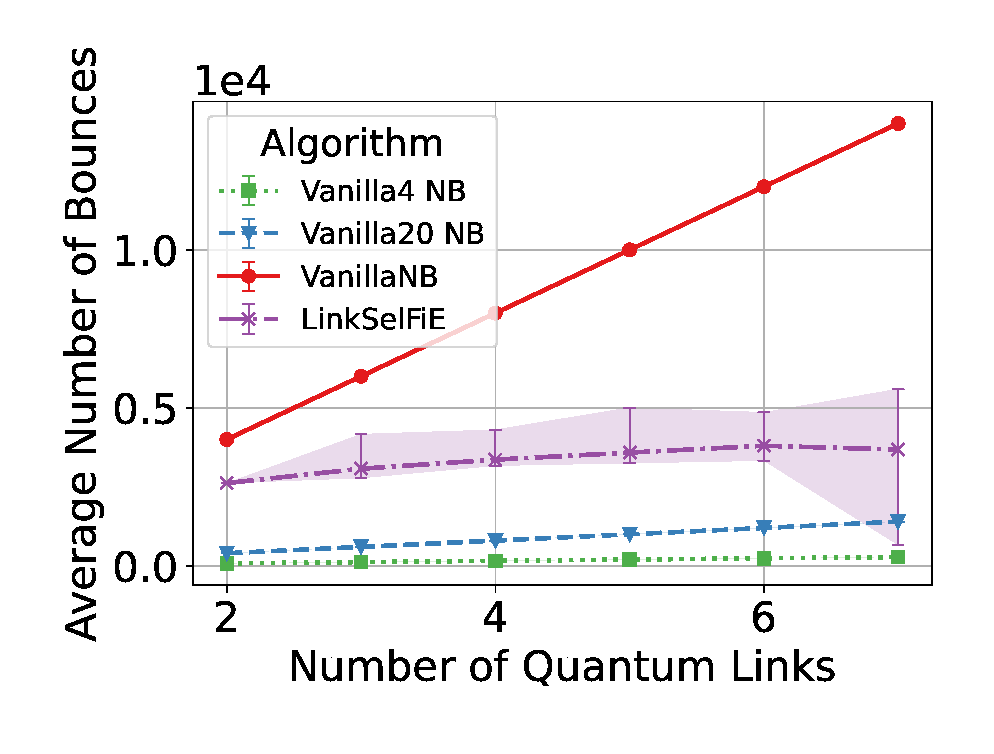
\includegraphics[width=0.45\columnwidth]{figure/plot_cost_vs_path_num_AmplitudeDamping.eps}
\caption{Amplitude Damping - Cost vs Path Number}
\label{fig:cost_amplitude}
\end{figure}

\begin{figure}[t]
\centering
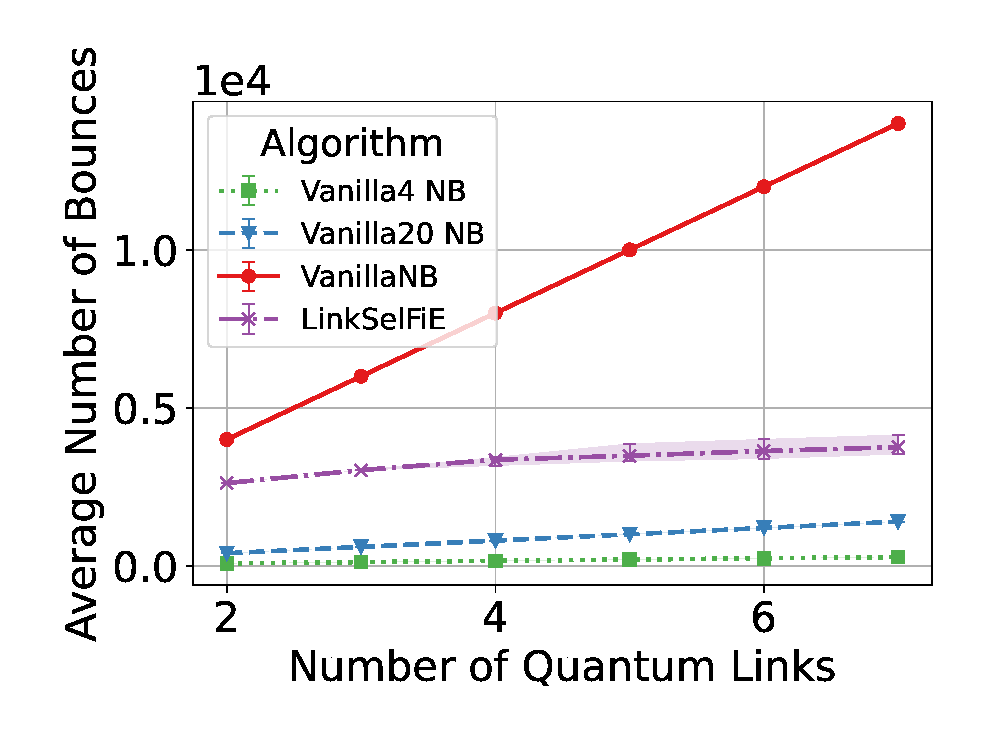
\includegraphics[width=0.45\columnwidth]{figure/plot_cost_vs_path_num_BitFlip.eps}
\caption{Bit-Flip - Cost vs Path Number}
\label{fig:cost_bitflip}
\end{figure}

\begin{figure}[t]
\centering
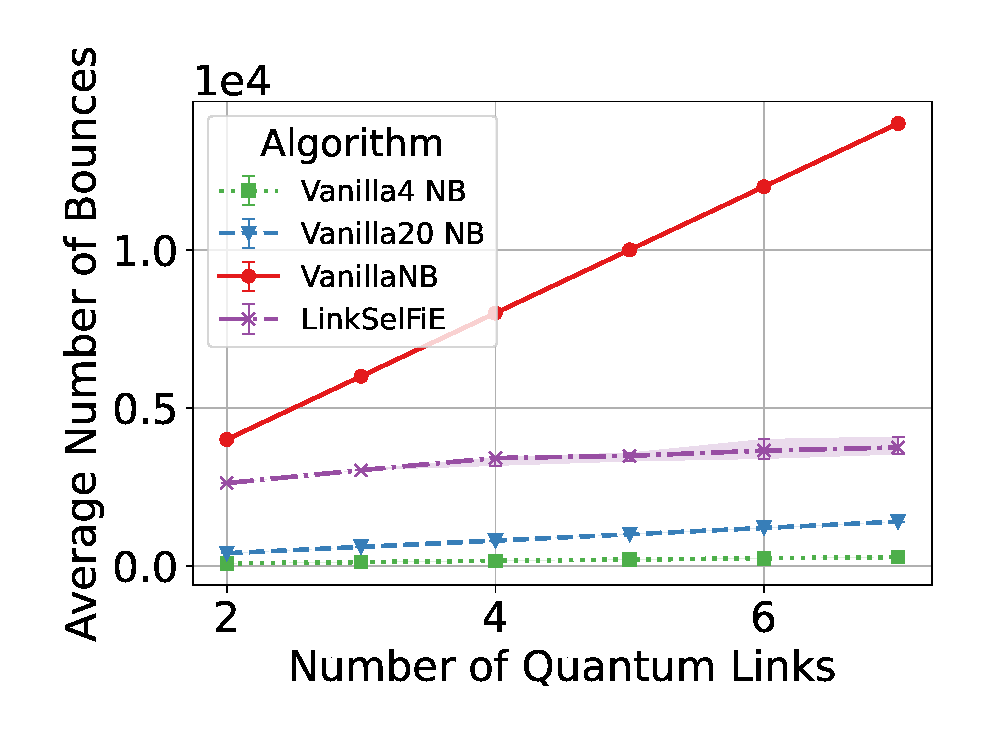
\includegraphics[width=0.45\columnwidth]{figure/plot_cost_vs_path_num_Dephase.eps}
\caption{Dephasing - Cost vs Path Number}
\label{fig:cost_dephase}
\end{figure}

\begin{figure}[t]
\centering
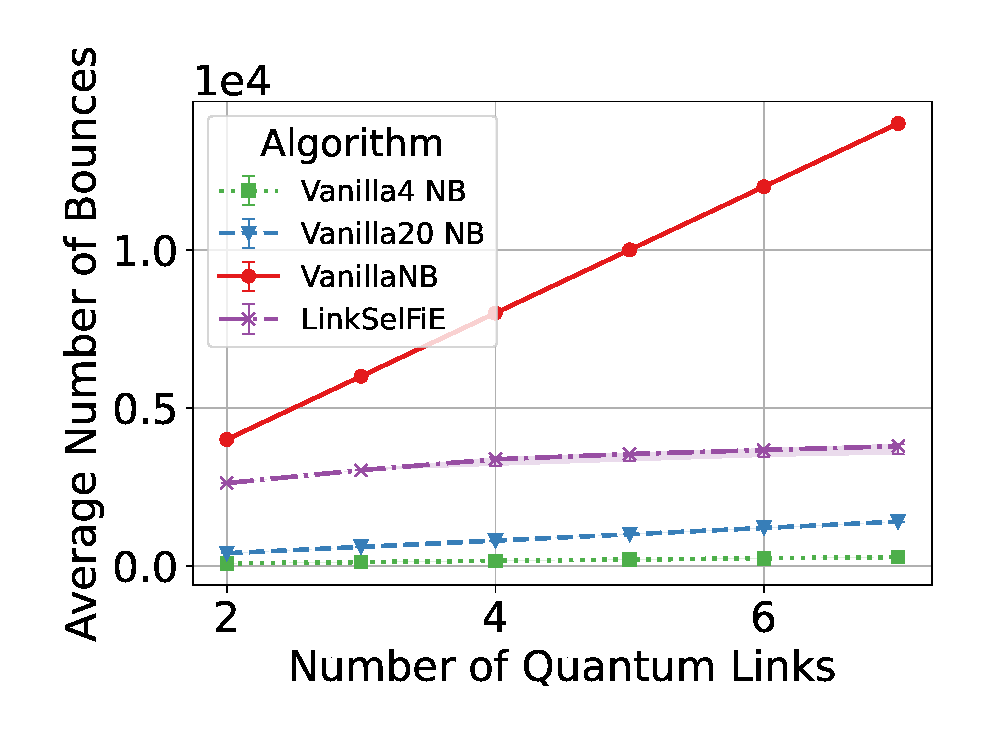
\includegraphics[width=0.45\columnwidth]{figure/plot_cost_vs_path_num_Depolar.eps}
\caption{Depolarizing - Cost vs Path Number}
\label{fig:cost_depolar}
\end{figure}

まず、これらのリンク選択アルゴリズムにおける量子リソース消費を評価する。
忠実度ギャップ Δ = 0.05 を固定し、複数の量子エンタングルメントリンクで
接続された2ノードの量子ネットワークをシミュレートする。それぞれのリン
クは、忠実度 1, 1 − Δ, 1 − 2Δ, …, 1 − (L − 1)Δ を持つものとする。その
後、各リンク選択アルゴリズムをネットワークに適用し、さまざまな L の値
に対してアルゴリズムが終了する際の量子リソース消費量を測定する。ここで、
量子リソース消費量の指標として総バウンス数を使用し、結果は 10 回の試行
の平均をとった。Vanilla 4NB、Vanilla 20NBがLinkSeLFiEよりも少ない資源
で配分できていることがわかる。バウンス数はL = 7のときにVanilla 20NB
でLinkSeLFiEの半分以下、Vanilla 4NBは1/10ほどである。


\begin{figure}[t]
\centering
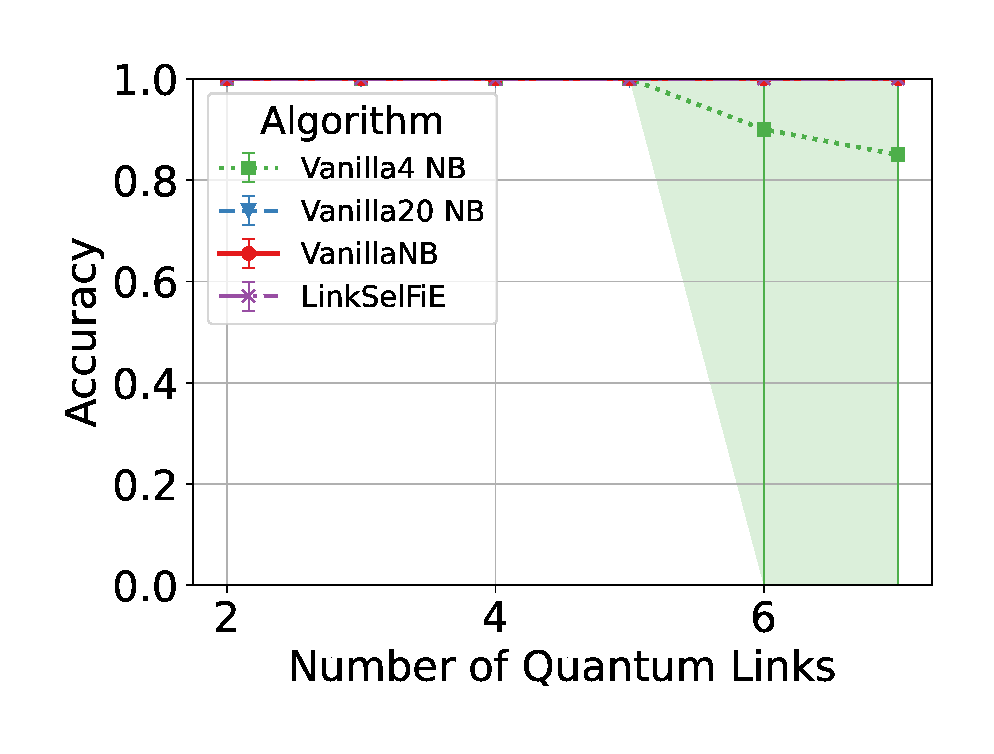
\includegraphics[width=0.45\columnwidth]{figure/plot_accuracy_vs_path_num_AmplitudeDamping.eps}
\caption{Amplitude Damping - Accuracy vs Path Number}
\label{fig:acc_amplitude}
\end{figure}

\begin{figure}[t]
\centering
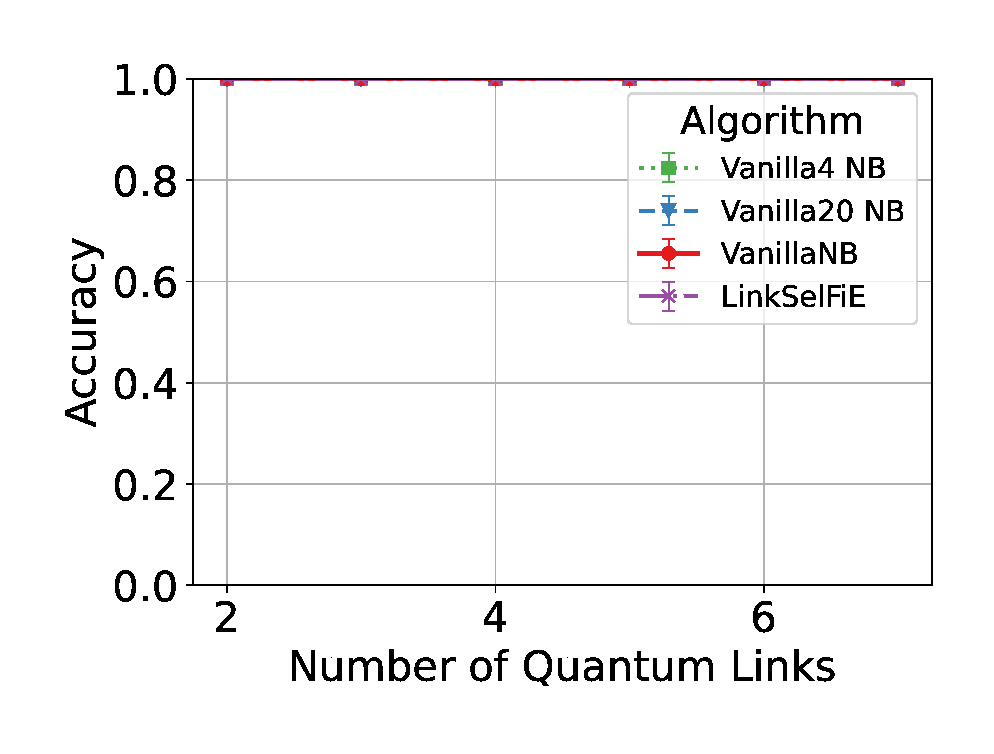
\includegraphics[width=0.45\columnwidth]{figure/plot_accuracy_vs_path_num_BitFlip.eps}
\caption{Bit-Flip - Accuracy vs Path Number}
\label{fig:acc_bitflip}
\end{figure}

\begin{figure}[t]
\centering
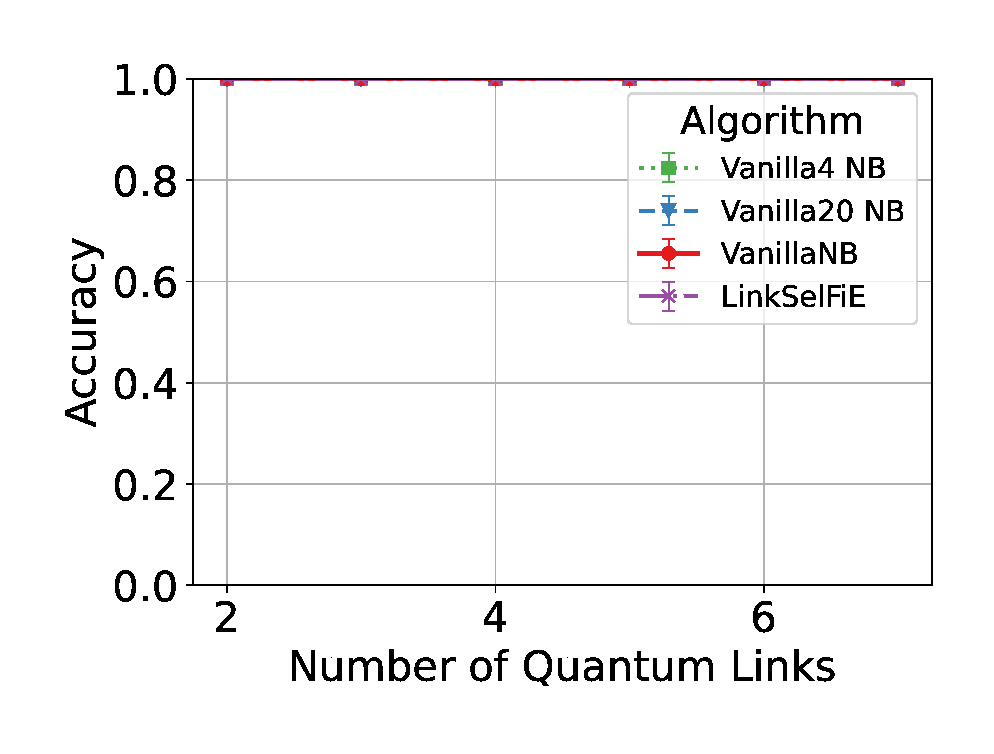
\includegraphics[width=0.45\columnwidth]{figure/plot_accuracy_vs_path_num_Dephase.eps}
\caption{Dephasing - Accuracy vs Path Number}
\label{fig:acc_dephase}
\end{figure}

\begin{figure}[t]
\centering
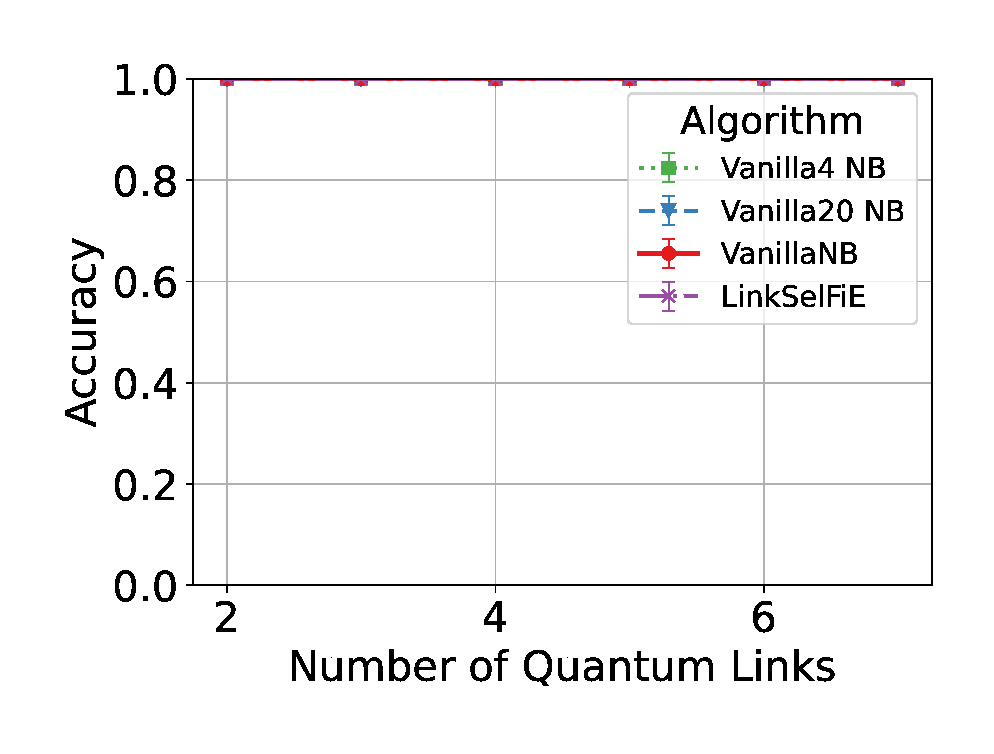
\includegraphics[width=0.45\columnwidth]{figure/plot_accuracy_vs_path_num_Depolar.eps}
\caption{Depolarizing - Accuracy vs Path Number}
\label{fig:acc_depolar}
\end{figure}

次に、リンク選択アルゴリズムにおける最適リンク判別率を評価する。忠実度
ギャップ Δ = 0.05 を固定し、複数の量子エンタングルメントリンクで接続さ
れた2ノードの量子ネットワークをシミュレートする。それぞれのリンクは、
忠実度 1, 1 − Δ, 1 − 2Δ, …, 1 − (L − 1)Δ を持つものとする。その後、各
リンク選択アルゴリズムをネットワークに適用し、さまざまな L の値に対し
てアルゴリズムの最適リンク判別率を測定する。ここで最適リンク判別率とは
アルゴリズムが真の忠実度が最大のリンクを正しく選択できた確率のことである。
結果は10 回の試行の平均をとった。Vanilla 4NB、Vanilla 20NBでは
LinkSeLFiEと同等の判別率があることがわかる。

\begin{figure}[t]
\centering
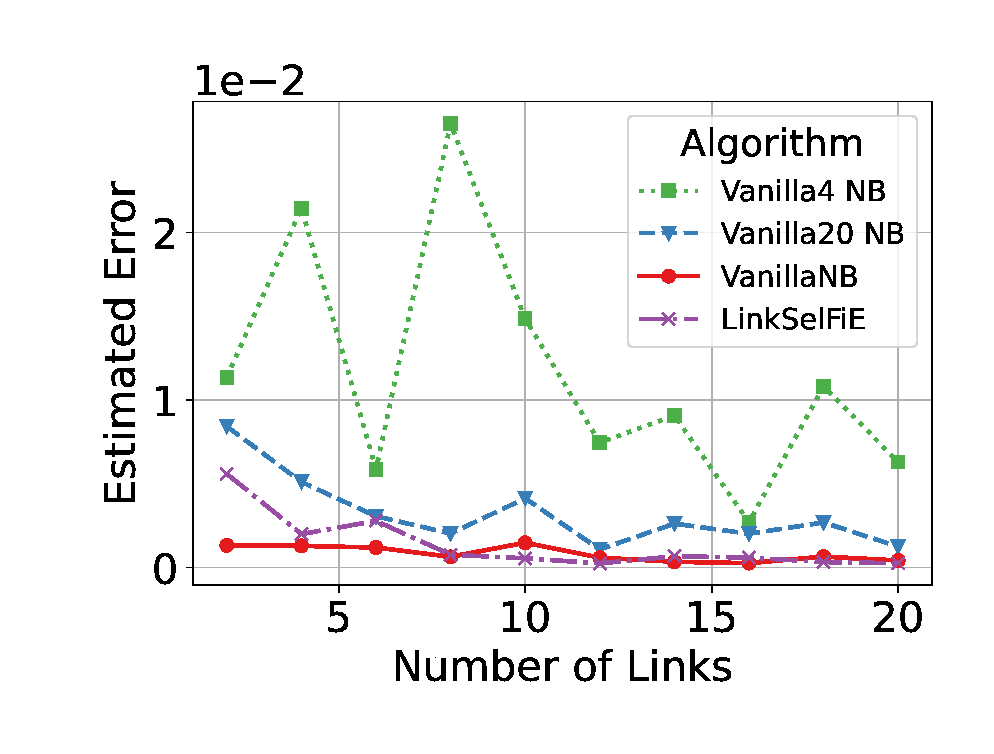
\includegraphics[width=0.45\columnwidth]{figure/plot_error_vs_path_num_AmplitudeDamping.eps}
\caption{Amplitude Damping - Estimation Error vs Path Number}
\label{fig:error_amplitude}
\end{figure}

\begin{figure}[t]
\centering
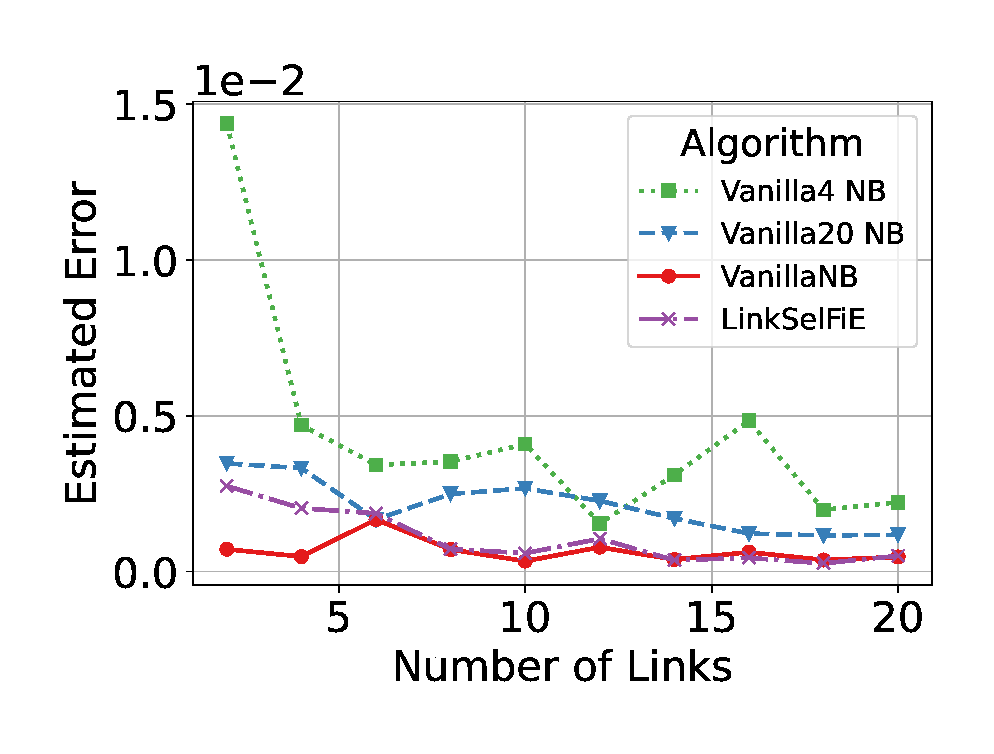
\includegraphics[width=0.45\columnwidth]{figure/plot_error_vs_path_num_BitFlip.eps}
\caption{Bit-Flip - Estimation Error vs Path Number}
\label{fig:error_bitflip}
\end{figure}

\begin{figure}[t]
\centering
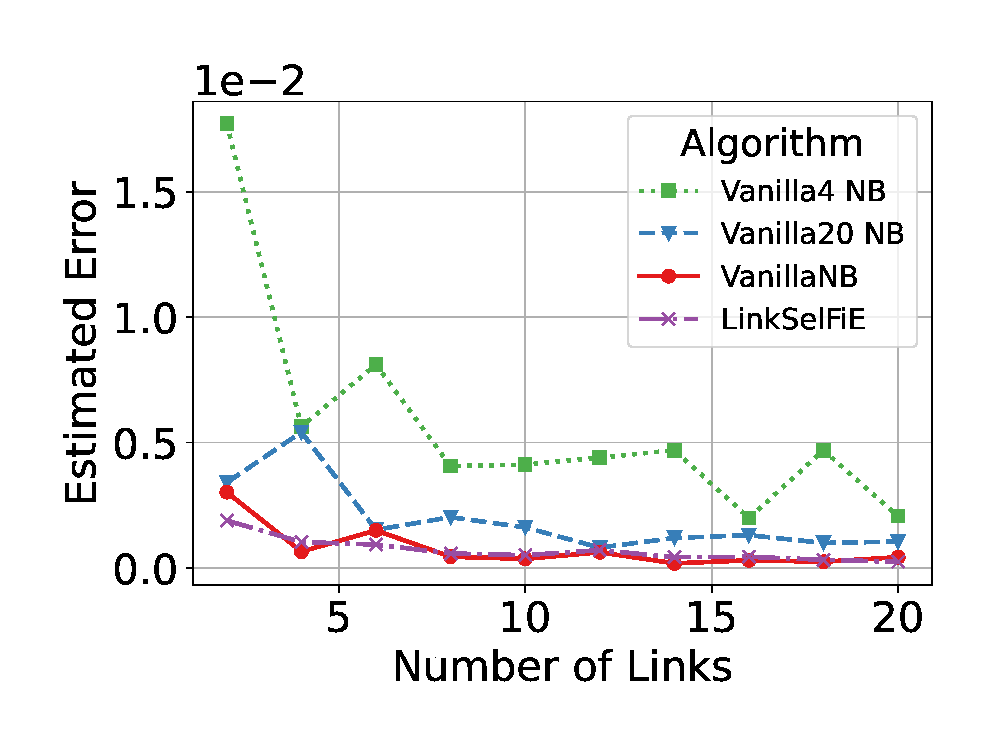
\includegraphics[width=0.45\columnwidth]{figure/plot_error_vs_path_num_Dephase.eps}
\caption{Dephasing - Estimation Error vs Path Number}
\label{fig:error_dephase}
\end{figure}

\begin{figure}[t]
\centering
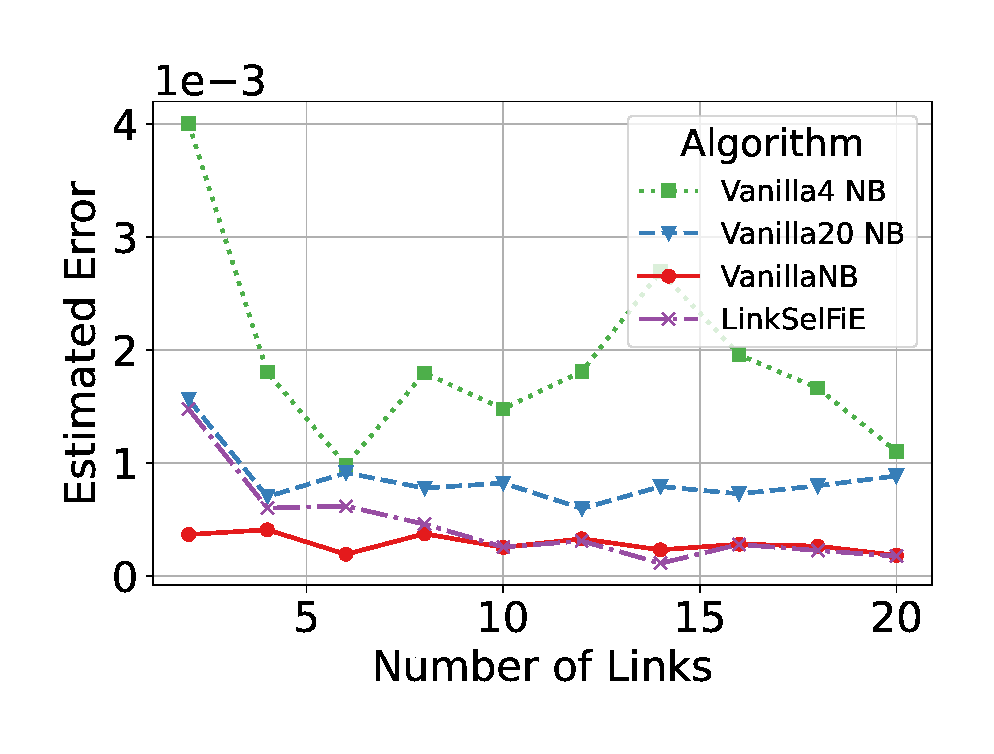
\includegraphics[width=0.45\columnwidth]{figure/plot_error_vs_path_num_Depolar.eps}
\caption{Depolarizing - Estimation Error vs Path Number}
\label{fig:error_depolar}
\end{figure}

\subsection{Fidelity Estimation Accuracy}
\label{sec:org0000b24}
次に、各アルゴリズムの忠実度推定精度を評価する。
各リンクの平均忠実度はそれぞれ \(\mu_1\) = 0.95 および \(\mu_i\) = 0.85(i = 2, 3, …, L)と設定する。
各リンク i の忠実度 \(f_i\) は、平均 \(\mu_i\)、分散 1/4 のガウス分布からサンプリングされる。
その後、各アルゴリズムをこのネットワークに適用し、
各アルゴリズムが選択した最適リンクの推定忠実度を得る。
アルゴリズムが出力した推定忠実度を、真の忠実度と比較することで、
相対誤差(relative error)を求める。
リンク数 L を 2 から 20 まで変化させ、
各設定について 10 回の試行を行い、その平均値を結果として出力する。

LinkSeLFiEの論文では"LinkSeLFiE の相対誤差は 1\% 未満であり、他のアルゴ
リズムと比較して有意な差は見られない。"と言及されていた。Vanilla 20NB
の相対誤差も1\% 未満であり、LinkSeLFiEと比較して有意な差は見られないと
言える。




\subsection{P(Point:結論の繰り返し)}
\label{sec:org2929232}
結果としてVanilla 20NBはLinkSeLFiEよりもはるかに少ないリソースで最適リ
ンクを選択しつつ、同等レベルの忠実度推定精度を達成しており、リンク判別
だけならばVanilla 4NBでもある程度判別可能であるということが分かった。
これは量子資源、最適リンクの特定、最適リンクの推定精度という観点で
LinkSeLFiEが均等配分手法を上回ることができていないことを示している。ゆ
えにLinkSeLFiEはアルゴリズムの資源効率性における優位性を示せていない。


\section{補足}
\label{sec:org7d6d641}
\subsection{LinkSeLFiEの目的}
\label{sec:orgf1f29e5}
\begin{itemize}
\item 最小限の量子資源で、最も高忠実度なリンクを特定し、その忠実度を正確に推定するアルゴリズムを設計する
\end{itemize}

"The main objective of this work is to efficiently estimate the fidelity of established entangled links."

"Our objective is to identify the link with the highest fidelity from a
link set and get its fidelity estimate while consuming as few quantum
resources as possible."

"Our algorithm deliberately considers the property of the network
benchmarking, with the objective of identifying the optimal
high-fidelity link from a link set with high confidence and consuming
as few resources as possible."

\subsection{相対誤差について言及している箇所}
\label{sec:org754424a}
As expected, LinkSeLFiE can not only identify the optimal link but
also evaluate its fidelity accurately. The relative error of
LinkSeLFiE is less than 1\%, which has no significant difference
compared with other algorithms.

誤差(relative error)1\%未満で他の手法と同程度としており、LinkSeLFiE
レベルの誤差(0.003)の必要性は書かれていない。


\subsection{実験で実証した内容}
\label{sec:org8034e77}
Moreover, we perform extensive simulations under
various scenarios to corroborate that L INK S EL F I E outperforms
other existing methods in terms of both identifying the optimal
link and reducing quantum resource consumption.

最適リンクの特定と量子資源消費の削減という両方の観点で、既存の他の手法
を上回ることを実証していると言っている

\subsection{VanillaNBの繰り返し回数Tについて言及している箇所}
\label{sec:orgacce58d}
"We compare our algorithm with two baselines, (1) the vanilla network
benchmarking algorithm (VanillaNB) and (2) the successive elimination
algorithm [27] (SuccElimNB).  VanillaNB uniformly benchmarks all the
quantum links for each bounce number with a fixed number of
repetitions T, which we set to T = 200 in our experiments.  SuccElimNB
invokes the network benchmarking subroutine with repetition times T =
4 …"




\subsection{ネットワークベンチマーキング(NB)について}
\label{sec:orgf4ad935}
NBは、量子ネットワークのパフォーマンスを測定するための基礎的な手法であ
る。特に、ネットワークのリンク品質を評価するために、量子状態の「バウン
ス」実験を繰り返すプロトコルが利用される。ネットワークベンチマーキング
は、あるリンクを通してエンタングルメントを生成し、その状態を送信ノード
S から受信ノード D に何度も往復(bounce)させることにより、リンクの
「生存確率(survival probability)」を測定する。

実際、1 つのベンチマーク実験は、次のパラメータによって特徴づけられる:
\begin{itemize}
\item M:バウンス回数の集合(例:\{1, 2, 3, 4\})
\item T:各バウンス回数に対する繰り返し回数(repetition times)
\end{itemize}
ベンチマークの過程で、各 m∈M に対して T 回の測定を行い、対応する生存確
率 bm を記録する。
これらの観測値 \{b\_m\} は、理論的に次のような指数減衰モデルに従う:


\[
b_m = A p^{2m},
\]
ここで,

\begin{itemize}
\item A:測定および状態準備エラーの影響を表す定数,
\item p:量子チャネルの脱分極パラメータ(depolarizing parameter)
\end{itemize}


このとき,pの推定値 \(\hat{p}\) から,
リンクの平均忠実度(average fidelity)は次式で求められる:
\[
\hat{F} = \frac{1 + \hat{p}}{2}.
\]

LinkSeLFiEの論文でNBは量子ネットワーク内のリンク品質を評価するための基
本的手続きとして説明されており、全ての手法(VanillaNB, SuccElimNB,
LinkSeLFiE)でこの NB をサブルーチンとして呼び出して動作する。

Network benchmarking (NB) is a fundamental procedure to evaluate the link quality in a quantum network.


\subsection{リンク数が大幅に増えるとVanilla 4NB,Vanilla 20NBはLinkSeLFiEよりも総バウンス数が増えるのか}
\label{sec:orgc515dd5}
\begin{itemize}
\item Vanilla20NB Yes
\item Vanilla4NB No
\end{itemize}

LinkSeLFiEは有望なリンクとそうでないリンクを判別するために最初に均等配
分を行なう。その際に4NBを全リンクに渡しているのでVanilla4NBよりも少な
い総バウンスになることはない。

\section{なぜこの話をするのか}
\label{sec:org95b3760}
ストーリー案に直結しているから。
ストーリー案の骨格
背景 量子ネットワークにおいて忠実度を高いリンクを効率的に判定する手法 LinkSelFiE が提案されている
動機 LinkSelFiE は通信需要を考慮していないが、現実には通信需要が高くかつ忠実度の高いリンクの判定が望まれる
目的 少ない計測 (バウンス) により利用率 x 忠実度が高いリンクの判定を可能とする

忠実度を高いリンクを効率的に判定する手法が均等配分で十分だとすると解く
価値の無い問題になってしまう。特にlinkselfieのように最大忠実度のリンク
を特定するのではなく、ある程度高い忠実度のリンクさえ分かればいいのなら
なおさら均等配分で良い。


\section{今後の方針}
\label{sec:org5bad211}
ストーリー案を修正するのか?
どのように?
\begin{itemize}
\item 均等配分ではうまくいかない状況(バウンスをたくさん使ってしまう状況)を考えなければいけない
\begin{itemize}
\item 測定精度が求められる状況
\end{itemize}
\item マルチホップにすると測定精度が要求される
\begin{itemize}
\item A - B - C - Dという経路でA - D間の測定誤差を1\%以内にするにはA - B
間、B - C間、C - D間での測定誤差は1\%よりも少なくしないといけない。
\item 忠実度は通信の成功率に依存しているのでA - D間で通信が成功するには、
A-B,B-C,C-D間全てで通信が成功しなければいけない。
\item QBGPという手法が既にある
\begin{itemize}
\item QBGPでは通信が確立された後のエンドツーエンドの量子通信が背景。つ
まり宛先が複数ありそれぞれに通信需要があるという拡張は自然ではな
いかもしれない
\end{itemize}
\end{itemize}
\end{itemize}
\end{document}